\documentclass[11pt]{exam}
\usepackage[utf8]{inputenc}
\usepackage[a4paper,top=2cm,left=2cm,right=2cm,bottom=2cm]{geometry}
\usepackage{import}
\usepackage[T1]{fontenc}
\usepackage[german,ngerman]{babel}
\usepackage[table]{xcolor}
\usepackage{amsthm, esvect}
\usepackage{mathtools}
\RequirePackage{amssymb, amsfonts, amsmath, latexsym, verbatim, xspace}
\usepackage{systeme}
\usepackage{multicol}
\usepackage{multirow}
\usepackage{framed}
\usepackage{array}
\usepackage{ragged2e}
\usepackage{graphicx}
\usepackage{pdflscape}
\usepackage{epstopdf}
\usepackage{booktabs}
\usepackage{pdfpages}
\usepackage{float} % Allows putting an [H] in \begin{figure} to specify the exact location of the figure
\usepackage{wrapfig} % Allows in-line images such as the example fish picture
\usepackage{tikz, graphicx} % tikz
\usepackage[position=top]{subfig}
\usepackage[bookmarks=true]{hyperref}%Links
\usepackage{enumerate}
\usepackage{enumitem}
\usepackage[german,ruled,vlined,linesnumbered,algosection]{algorithm2e}
\usepackage[labelfont=sf]{caption}
\usepackage{lmodern}
\usepackage{lscape}
\usepackage{tabularx}
\usepackage{systeme}
\usepackage{hhline}
\usepackage{subfiles}
\usepackage{stackengine}
\usepackage{setspace}
\usepackage{MnSymbol}
\usepackage{tcolorbox}
\usepackage{bbm}
\usepackage{url}
\usepackage{xparse}
\usepackage{sectsty}
\usepackage{array}
\usepackage{ragged2e}
\usepackage{listings} %Stellt Code-Snippets sauber dar

% definiert die Sprache
\selectlanguage{German}

% add command for different dates in Swiss fashion
\newcommand{\monthwordlong}[1]{\ifcase#1 \or Januar\or Februar\or März\or April\or Mai\or Juni\or Juli\or August\or September\or Oktober\or November\or Dezember\fi}
\newcommand{\monthwordshort}[1]{\ifcase#1\or Jan\or Feb\or Mar\or Apr\or Mai\or Jun\or Jul\or Aug\or Sept\or Okt\or Nov\or Dez\fi}
\newcommand{\datelong}{\number\day.\:\monthwordlong{\the\month}\:\number\year}
\newcommand{\dateshort}{\number\day.\:\monthwordshort{\the\month}\:\number\year}

% define color of links inside a text
\definecolor{linkblue}{RGB}{0, 0, 80}
\definecolor{plotblue}{RGB}{100, 100, 255}
\definecolor{myblue}{RGB}{8,164,214}
\definecolor{myred}{RGB}{143,42,41}
\definecolor{forestgreen}{RGB}{34,139,34}
\definecolor{highdive}{RGB}{10,169,194}
\definecolor{charcoal}{RGB}{74,74,74}
\hypersetup{
	colorlinks=true,
	linkcolor=linkblue,
	filecolor=magenta,
	urlcolor=plotblue,
	citecolor=linkblue,
	pdfpagemode=FullScreen,
}


\lstdefinestyle{mystyle}{ % definiert den style des Code-Snippets
	%backgroundcolor=\color{backcolour},
	%commentstyle=\color{codegreen},
	%keywordstyle=\color{magenta},
	%numberstyle=\tiny\color{codegray},
	%stringstyle=\color{codepurple},
	basicstyle=\ttfamily\footnotesize,
	breakatwhitespace=false,
	breaklines=true,
	captionpos=b,
	keepspaces=true,
	%numbers=left,
	%numbersep=5pt,
	showspaces=false,
	showstringspaces=false,
	showtabs=false,
	tabsize=4
}
\lstset{style=mystyle}
\pagestyle{foot}
\firstpagefooter{}{}{}
\runningfooter{}{}{Seite \thepage\:von \numpages}
\runningfootrule
\linespread{1.15} % Line spacing

%Exam Konfiguration
\qformat{\textbf{Aufgabenstellung:}}
\hqword{Frage:}
\hpword{Mögliche Punkte:}
\hsword{Erreicht:}
\htword{Total:}
\pointpoints{Punkt}{Punkte}
\renewcommand*\half{.5}
\renewcommand{\solutiontitle}{}
\shadedsolutions

\def\bl{\begin{solution}} %\bl für Beginn Lehrerkommentar
\def\el{\end{solution}} %\el für Ende Lehrerkommentar

% Inhaltsverzeichnis definieren
\renewcommand{\contentsname}{Aufgabenübersicht}


% definiert die Blöcke pro Aufgabe
\newcommand{\derBereich}{}
\def\bereich#1{
	\renewcommand\derBereich{#1}}
\newcommand{\derTitel}{}
\def\titel#1{
	\renewcommand\derTitel{#1}}


% definiert die Farbe der Themenbereiche
\ExplSyntaxOn
% Funktion: wendet direkt die textfarbe an
\cs_new_protected:Npn \apply_color:nn #1 #2 {
	\str_case:nnF {#1}{
		{Integral}			{ \textcolor{orange}{#2} }
		{Differential}		{ \textcolor{green}{#2} }
		{Vektor}			{ \textcolor{cyan}{#2} }
		{Stochastik}		{ \textcolor{yellow}{#2} }
		{FolgenReihen}		{ \textcolor{brown}{#2} }
		{Wachstum}			{ \textcolor{magenta}{#2} }
	}{ \textcolor{black}{#2} }
}

\NewDocumentCommand{\colortext}{mm}{
	\apply_color:nn {#1} {#2}
}

% Funktion: wendet direkt die die cellfarbe an
\cs_new_protected:Npn \apply_cellcolor:n #1 {
	\str_case:VnF {#1}{
		{Integral}			{ \cellcolor{orange} }
		{Differential}		{ \cellcolor{green} }
		{Vektor}			{ \cellcolor{cyan} }
		{Stochastik}		{ \cellcolor{yellow} }
		{FolgenReihen}		{ \cellcolor{brown} }
		{Wachstum}			{ \cellcolor{magenta} }
	}{ \cellcolor{black} }
}

\NewDocumentCommand{\colorcell}{m}{
	\apply_cellcolor:n {#1}
}
\ExplSyntaxOff

%===================================================
% setzt die Blöcke der einzelnen Aufgaben
\newcounter{numquestion}
\renewcommand{\thenumquestion}{\arabic{numquestion}}
\newenvironment{aufgabe}{
	\refstepcounter{numquestion}
	\newpage
	\addcontentsline{toc}{section}{\colortext{\derBereich}{\textbf{\thenumquestion.~ \derBereich: }}\derTitel}

	\begin{center}
		\begin{tabular}[width=\textwidth]{|c | p{11cm} | p{4cm} |}
			\hline
			\parbox[0pt][2.5em][c]{0cm}{}\LARGE\textbf{\thenumquestion} & \large\textbf{\derTitel} &  \colorcell{\derBereich} \derBereich\\ \hline
		\end{tabular}
	\end{center}

	\begin{questions}
		\question
	}{
	\end{questions}
}


%===================================================
\newenvironment{itemcols}[1][]{
	\begin{itemize}\begin{multicols}{#1}
		}{
	\end{multicols}\end{itemize}
}
%%
% Math Arrows
%%
\newcommand{\same}{\ensuremath{\Longleftrightarrow}}
\renewcommand{\to}{\ensuremath{\longrightarrow}}
\newcommand{\qsame}{\quad\same\quad}
\newcommand{\dsame}{\ensuremath{:\Leftrightarrow}}
\newcommand{\qdsame}{\quad\dsame\quad}
\newcommand{\ldsame}{\ensuremath{:\Longleftrightarrow}}
\newcommand{\samedef}{\ensuremath{\us {\text{def}} \Leftrightarrow}}
\newcommand{\qsamedef}{\quad\samedef\quad}
\newcommand{\lsamedef}{\ensuremath{\us {\text{def}} \Longleftrightarrow}}
\newcommand{\qlsamedef}{\quad\lsamedef\quad}


%%
% Mengendefinitionen
%%
\newcommand{\M}{\ensuremath{\mathcal{M}}}
\newcommand{\N}{\ensuremath{\mathbb{N}}}
\newcommand{\Z}{\ensuremath{\mathbb{Z}}}
\newcommand{\Q}{\ensuremath{\mathbb{Q}}}
\newcommand{\I}{\ensuremath{\mathbb{I}}}
\newcommand{\R}{\ensuremath{\mathbb{R}}}
\newcommand{\C}{\ensuremath{\mathbb{C}}}
\renewcommand{\S}{\ensuremath{\mathbb{S}}}
\newcommand{\Prim}{\ensuremath{\mathbb{P}}}
\newcommand{\0}{\ensuremath{\emptyset}}
\renewcommand{\Re}{\ensuremath{\operatorname{Re}}}
\renewcommand{\Im}{\ensuremath{\operatorname{Im}}}
\newcommand{\strich}{\ensuremath{\big\vert}}

%%
% Mengenoperation
%%
\renewcommand{\nin}{\not\in}


%%
% Logisches Und und Oder
%%
\newcommand{\sand}{\ensuremath{\; \land \;}}
\newcommand{\sor}{\ensuremath{\; \lor \;}}
\renewcommand{\*}{\ensuremath{\cdot}}
\newcommand{\oder}{\vee}
\newcommand{\n}{\neg}
\newcommand{\und}{\wedge}


%%
% Bei Integral, Summe,... die Grenzen über bzw.
% unter das Zeichen
%%
\renewcommand{\d}[1]{\ensuremath{\operatorname{d}\!{#1}}}
\newcommand{\Sum}{\sum\limits}
\newcommand{\Prod}{\prod\limits}
\newcommand{\Min}{\min\limits}
\newcommand{\Max}{\max\limits}
\newcommand{\Lim}{\lim\limits}
\newcommand{\Inf}{\inf\limits}
\newcommand{\Sup}{\sup\limits}
\newcommand{\Liminf}{\liminf\limits}
\newcommand{\Limsup}{\limsup\limits}
%\renewcommand{\Cup}{\bigcup\limits}
%\renewcommand{\Cap}{\bigcap\limits}
\newcommand{\Otimes}{\bigotimes\limits}
\newcommand{\Oplus}{\bigoplus\limits}


%%
% Arcus Cotangens, Logarithmus
%%
\let\oldsin\sin
\renewcommand{\sin}[1]{\oldsin{\left(#1\right)}}
\let\oldcos\cos
\renewcommand{\cos}[1]{\oldcos{\left(#1\right)}}
\let\oldtan\tan
\renewcommand{\tan}[1]{\oldtan{\left(#1\right)}}
\let\oldarcsin\arcsin
\renewcommand{\arcsin}[1]{\oldarcsin{\left(#1\right)}}
\let\oldarccos\arccos
\renewcommand{\arccos}[1]{\oldarccos{\left(#1\right)}}
\let\oldarctan\arctan
\renewcommand{\arctan}[1]{\oldarctan{\left(#1\right)}}
\let\oldln\ln
\renewcommand{\ln}[1]{\oldln{\left(#1\right)}}
\newcommand{\Log}[2]{\ensuremath{\operatorname{log}_{#1}\left(#2\right)}}
\newcommand{\e}{\operatorname{e}}
\renewcommand{\exp}[1]{\ensuremath{\operatorname{\e}^{#1}}}


%%
% Griechische Buchstaben
%%
\renewcommand{\epsilon}{\ensuremath{\varepsilon}}
\renewcommand{\phi}{\varphi}
\renewcommand{\l}{\lambda}
\renewcommand{\t}{\tau}


%%
% Bezeichnungen
%%
\newcommand{\Rgn}{\R_{>0}} % R grösser Null
\newcommand{\Rad}{\operatorname{Rad}}   % Radikal
\newcommand{\kgV}{\operatorname{kgV}}   % Kleinster gemeinsame Vielfache
\newcommand{\ggT}{\operatorname{ggT}}   % Grösster gemeinsame Teiler
\newcommand{\winkel}{\sphericalangle}          % Winkelsymbol
\DeclarePairedDelimiter\abs{\lvert}{\rvert} % besserer Betrag
\makeatletter
\let\oldabs\abs
\def\abs{\@ifstar{\oldabs}{\oldabs*}}
\makeatother


%%
% Vektorgeometrie
%%
\renewcommand{\v}[1]{\vv{#1}}       % besserer Pfeil über Buchstaben
\renewcommand{\vec}[2]{\begingroup\renewcommand{\arraystretch}{1}\left(\begin{array}{c} #1 \\ #2 \end{array}\right)\endgroup}   % two dimensional vector
\renewcommand{\Vec}[3]{\begingroup\renewcommand{\arraystretch}{1}\left(\begin{array}{c} #1 \\ #2 \\ #3 \end{array}\right)\endgroup}      % three dimensional vector


%%
% Text
%%
\newcommand*{\Ueq}[1]{\mathrel{\mathop{=}\limits_{\text{#1}}}}
\newcommand*{\Oeq}[1]{\mathrel{\stackrel{\text{#1}}{=}}}
\newcommand{\utext}[2]{\underbrace{#1}_{\substack{#2}}}
\newcommand{\otext}[2]{$\overbrace{\textrm{#1}}^{\textrm{#2}}$}
\newcommand{\lineortext}[1]{\hspace{0,1cm}\underline{\hspace{0.1cm}\hphantom{#1}\hspace{0.1cm}}\hspace{0,1cm}} % Lückentext erstellen
\newcommand{\gap}[1]{\rule{#1 cm}{1pt}}
\graphicspath{{images/}}
%=========================================================
\newcommand{\school}{KS Heerbrugg}
\newcommand{\fach}{Mündliche Matura Mathematik}
\newcommand{\teacher}{Jonas Guler}
\newcommand{\myyear}{2026}
\newcommand{\mastertitle}{Prüfungskatalog}
%=========================================================
\fontsize{12}{12}\selectfont
%definiert die Version
\printanswers % falls kommentiert werden die Schülerversionen angezeigt
%=========================================================
\begin{document}
\noindent
\begin{small}
	\begin{tabular*}{\textwidth}{l @{\extracolsep{\fill}}l @{\extracolsep{7pt}}l}
		\fach & & \teacher\\
		\school & & \myyear\\
	\end{tabular*}
\end{small}
\vspace{0.75cm}\\
\rule[1ex]{\textwidth}{1pt}
\begin{center}
	{\bf\huge\mastertitle}\\
\end{center}
\rule[1ex]{\textwidth}{1pt}\\
\tableofcontents
%=========================================================
%-------------------TESTFRAGEN
%=========================================================
\bereich{Differential}
\titel{Ableitung, Stammfunktion}
\begin{aufgabe}
	Der abgebildete Graph zeigt drei Funktionen des Typs $f(x)=x^k$ für $k\in\Z$.\\
	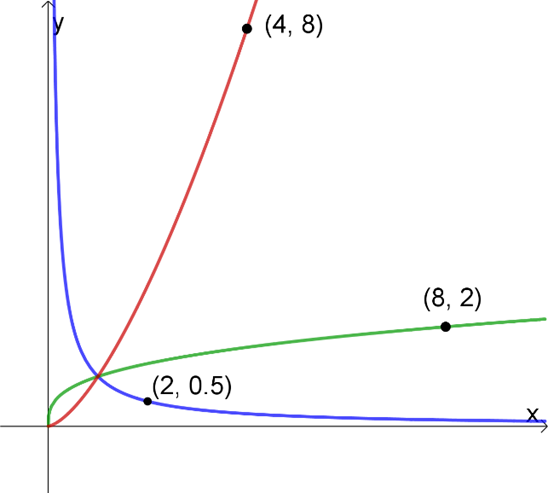
\includegraphics[width=0.4\textwidth]{divexpgraph.png}
	\begin{parts}
		\part Skizziere den Graphen der Ableitung der blauen Funktion.\\
		\begin{tikzpicture}[x=10mm, y=10mm, >=latex, font= \footnotesize, scale=0.6]
			%Raster zeichnen
			%\draw [color=gray!50]  [step=10mm] (-4.3,-4.3) grid (4.3,4.3);
			% Achsen zeichnen
			\draw[->,thick] (-1.3,0) -- (6.8,0) node[right, below] {\normalsize $x$};
			\draw[->,thick] (0,-1.3) -- (0,6.8) node[above, left] {\normalsize $y$};
			% Achsen beschriften
			%\foreach \x in {-4,...,-2,-1,1,2,...,4} \draw (\x,-.1) -- (\x,.1) node[below=4pt] {$\x$};
			%\foreach \y in {-4,...,-2,-1,1,2,...,4} \draw (-.1,\y) -- (.1,\y) node[left=4pt] {$\y$};
			% Besserer Ursprung
			%\draw[color=black] (0pt,-7pt) node[right] {$0$};
			%Funktionen zeichnen:
			%\clip(-4.3,-4.3) rectangle (4.3,4.3); %Bildbereich
			%Beschriftung
			%\node[myred]  at (3.1,-2.3) {$f$};
		\end{tikzpicture}
		\part Benutze die eingezeichneten Punkte, um die Funktionsgleichungen jedes Graphen zu bestimmen.
		\bl \[8=4^k \Leftrightarrow 2^3=2^{2k}\Leftrightarrow k=1.5\]\[ rot(x)=x^{1.5}\quad grün(x)=x^\frac{1}{3}\quad blau=x^{-1}\] \el
		\part Berechne die Ableitung und die Stammfunktion der blauen Funktion.
		\bl \[f'(x)=-x^{-2} \quad F(x)=\ln{x}\] \el
		\bl
		\part Der rote und grüne Graph umschliessen eine Fläche im ersten Quadranten. Erkläre, wie diese Fläche berechnet werden kann.
		\part Die eingeschlossene Fläche wird nun um die $x-$Achse rotiert. Erkläre die Idee, wie das Rotationsvolumen berechnet werden kann.
		\part Vergleichen wir zwei Funktionen des Typs $f(x)=x^2$ und $g(x)=2^x$. Welche wächst schneller? Begründe deine Antwort graphisch.
		\el
	\end{parts}
\end{aufgabe}

%

\bereich{Vektor}
\titel{Gerade, Durchstosspunkt, Abstand}
\begin{aufgabe}
	Gegeben ist die Gleichung einer Gerade ${g:\v{r}=\Vec{-7}{3}{3}+t\*\Vec{4}{1}{-1}}$.
	\begin{parts}
		\part Erkläre die Idee hinter dieser Beschreibung einer Gerade. Welche Elemente der Gleichung beschreiben was?
		\bl Stützvektor und Richtungsvektor \el
		\part Ist $g$ parallel zu einer Koordinatenachse oder einer Grundebene des Koordinatensystems? Begründe deine Antwort.
		\bl Betrachte den Richtungsvektor, da weder eine noch zwei Nullen enthalten sind, ist dieser nicht parallel. \el
		\part Wähle eine Grundebene und berechne den Durchstosspunkt der Gerade $g$.
		\bl $xy-$Ebene: $Z=0 \Rightarrow 3-t=0 \Rightarrow t=3$. Das heisst, der Durchstosspunkt liegt bei $D(5\mid6\mid0)$\el
		\part Wir möchten den Punkt auf der Gerade bestimmen, der den Kürzesten Abstand zum Ursprung aufweist. Erkläre, wie du diesen Punkt findest?
		\bl \begin{align*}E:4x+y-z&=0\\ \Leftrightarrow-28+16t+3+t-3+t&=0 \Leftrightarrow t=\frac{14}{9}\\ &\Rightarrow D(5.44\mid4.56\mid1.44)\end{align*}
		\part Wie sieht die Gleichung einer Gerade aus die parallel zur $z-$Achse oder $xy-$Ebene verläuft?\el
	\end{parts}
\end{aufgabe}


%----------------------------------------------------------


\bereich{Integral}
\titel{Flächen}
\begin{aufgabe}
	\begin{minipage}{0.6\linewidth}
		\begin{parts}
			\part Der Graph auf der linken Seite zeigt eine Parabel $f$. Wie lautet die Funktionsgleichung?
			\bl \[\Rightarrow f(x)=\frac{1}{2}x^2-x-\frac{3}{2}\] \el
			\part Erkläre, was die Stammfunktion von $f$ beschreibt?\\ Skizziere die Stammfunktion von $f$ im Graphen rechts.
		\end{parts}
	\end{minipage}
	\hfill
	\begin{minipage}{0.375\linewidth}
		\centering
		\begin{tikzpicture}[x=10mm, y=10mm, >=latex, font= \footnotesize, scale=0.6]
			%Raster zeichnen
			\draw [color=gray!50]  [step=10mm] (-3.3,-3.3) grid (5.3,3.3);
			% Achsen zeichnen
			\draw[->,thick] (-3.3,0) -- (5.8,0) node[right, below] {\normalsize $x$};
			\draw[->,thick] (0,-3.3) -- (0,3.8) node[above, left] {\normalsize $y$};
			% Achsen beschriften
			\foreach \x in {-3,-2,-1,1,2,...,5} \draw (\x,-.1) -- (\x,.1) node[below=4pt] {$\x$};
			\foreach \y in {-3,-2,-1,1,2,3} \draw (-.1,\y) -- (.1,\y) node[left=4pt] {$\y$};
			% Besserer Ursprung
			\draw[color=black] (0pt,-7pt) node[right] {$0$};
			%Funktionen zeichnen:
			\clip(-3.3,-3.3) rectangle (5.3,3.3); %Bildbereich
			\draw[plotblue,thick,domain=-3:5,samples=200] plot (\x, {0.5*(\x+1)*(\x-3)});
			%Beschriftung
			%\node[myred]  at (3.1,-2.3) {$f$};
		\end{tikzpicture}
	\end{minipage}
	\begin{parts}
		\setcounter{partno}{2}
		\part Berechne die eingeschlossene Fläche zwischen dem Graphen und der $x-$Achse.
		\bl \begin{align*} \int f(x)\d{x}=\frac{1}{6}x^3-\frac{1}{2}x^2-\frac{3}{2}x\\ \int_{-1}^{3} f(x)\d{x}=-\frac{16}{3}	\end{align*} \el
		\part Warum ist das Integral negativ? Erkläre.
		\bl Integral ist eine unendliche Summe von unendlich kleinen Rechtecken, wobei die Höhe gleich dem Funktionswert sind. Falls die Funktion unterhalb der $x-$Achse verläuft ist also die Höhe negativ und ergo das Integral ist negativ. \el
		\part Wie gehst du in der Berechnung der eingezeichneten Fläche vor?\\
		\begin{minipage}{0.4\linewidth}
			\begin{tikzpicture}[x=10mm, y=10mm, >=latex, font= \footnotesize, scale=0.6]
				%Raster zeichnen
				\draw [color=gray!50]  [step=10mm] (-3.3,-3.3) grid (5.3,3.3);
				% Achsen zeichnen
				\draw[->,thick] (-3.3,0) -- (5.8,0) node[right, below] {\normalsize $x$};
				\draw[->,thick] (0,-3.3) -- (0,3.8) node[above, left] {\normalsize $y$};
				% Achsen beschriften
				\foreach \x in {-3,-2,-1,1,2,...,5} \draw (\x,-.1) -- (\x,.1) node[below=4pt] {$\x$};
				\foreach \y in {-3,-2,-1,1,2,3} \draw (-.1,\y) -- (.1,\y) node[left=4pt] {$\y$};
				% Besserer Ursprung
				\draw[color=black] (0pt,-7pt) node[right] {$0$};
				%Funktionen zeichnen:
				\clip(-3.3,-3.3) rectangle (5.3,3.3); %Bildbereich
				\draw[plotblue,thick,domain=-3:5,samples=200] plot (\x, {0.5*(\x+1)*(\x-3)});
				\draw[plotblue,thick,domain=-3:5,samples=200] plot (\x, {2*\x-2});
				% Bereich unter Funktionen einfärben
				\fill[plotblue, fill opacity=0.3] plot[domain=0.17157:3] (\x,{0.5*(\x+1)*(\x-3)}) -- plot[domain=1:0.17157] (\x,{2*\x-2}) -- cycle;
				%Beschriftung
				%\node[myred]  at (3.1,-2.3) {$f$};
			\end{tikzpicture}
		\end{minipage}
		\hfill
		\begin{minipage}{0.575\linewidth}
			\bl\begin{align*} A&=\abs{\int_{1}^{3} f(x)\d{x}} + \abs{\int_{0.17157}^{1} f(x)-g(x)\d{x}}\\&= \frac{8}{3}+0.876 = 3.543 \end{align*}\el
		\end{minipage}
		\bl \part Wie lautet die Funktionsgleichung, wenn der Graph $5$ Einheiten nach oben und $3$ Einheiten nach rechts verschoben wird?\\
		Wie lautet die Funktionsgleichung, wenn der Graph an der $x-$Achse gespiegelt wird? \el
	\end{parts}
\end{aufgabe}

%

\bereich{Vektor}
\titel{Durchstosspunkt und Schnittwinkel}
\begin{aufgabe}
	Die Gerade ${g:\v{r}=\Vec{-4}{-10}{8}+t*\Vec{2}{3}{-2}}$ und die Ebene $E:3x-y+4z-15=0$ sind gegeben.
	\begin{parts}
		\part Welche gegenseitige Lage können eine Gerade und eine Ebene im Raum einnehmen?
		\bl g parallel zu E: Richtungsvektor senkrecht zu Normalvektor\\ g in E: parallel und Stützpunkt von g gehört zu E\\ Schneidend: Durchstosspunkt berechnen \el
		\part Erkläre, welcher Winkel als \flqq Zwischenwinkel zwischen einer Gerade und einer Ebene\frqq\: angesehen wird.
		\part Welches Werkzeug wird für die Winkelberechnung in der Vektorgeometrie benutzt. Wende dieses auf das obige Problem an.
		\bl \[\cos{\phi}=\frac{\Vec{3}{-1}{4}\*\Vec{2}{3}{-2}}{\sqrt{9+1+16}\*\sqrt{4+9+4}}=\frac{6-3-8}{\sqrt{26}\*\sqrt{17}} \Rightarrow \phi=103.758^\circ\] \el
		\part Welche anderen Möglichkeiten haben wir Ebenen im Raum zu beschreiben?
		\bl Parametergleichung bestehend aus einem Stützpunkt und zwei nicht kollinearen Richtungsvektoren \el
		\part Betrachte den Stützpunkt der Gerade $g$. Wie weit ist der Punkt von der Ebene $E$ entfernt? Erkläre den Lösungsweg, ohne direkt die Formel zu verwenden.
		\bl Benutze den Normalvektor um eine Senkrechte durch $P$ zu legen $\Rightarrow$ Berechne den Durchstosspunkt S $\Rightarrow$ Berechne die Länge des Vektors $\v{PS}$
		\part Einige Fragen zur Lage der Ebene $E$:
		\begin{itemize}
			\item Ist der Ursprung Teil der Ebene $E$? $\Rightarrow$ Nein, d müsste 0 sein.
			\item Wie schaut die Koordinatengleichung einer Ebene aus, die parallel zur $xy-$Ebene ist? $\Rightarrow z=$Zahl
			\item Wie schaut die Koordinatengleichung einer Ebene aus, die parallel zur $x-$Achse ist? $\Rightarrow$ $x$ müsste in der Koordinatengleichung fehlen.
		\end{itemize}\el
	\end{parts}
\end{aufgabe}


%----------------------------------------------------------


\bereich{Integral}
\titel{Fläche unter Kurve}
\begin{aufgabe}
	Gegeben ist der Graph einer Funktion $f(x)=\sqrt{x}$ und ein Rechteck $ABCD$ mit den Eckpunkten $A(1\mid0), B(4\mid0), C(4\mid2)$ und $D(1\mid2)$.\\
	\begin{minipage}{0.6\linewidth}
		\begin{parts}
			\part Skizziere den Graph und das Rechteck. Wie kannst du den prozentualen Anteil des Rechtecks bestimmen, der unterhalb des Graphen liegt?
			\bl\begin{align*} T&=\int_{1}^{4}\sqrt{x}\d{x}=\left.\frac{2}{3}x^{\frac{3}{2}}\right\vert_1^4=\frac{16}{3}-\frac{2}{3}=\frac{14}{3}\\&\Rightarrow \text{Anteil:} \frac{\frac{14}{3}}{6}\*100=77\%\end{align*} \el
			\part Stell dir eine Parallele zur $y-$Achse vor, die die Fläche unterhalb des Graphen im Rechteck halbiert. Wie kannst du die $x-$Stelle finden, an der sich diese vertikale Linie befindet.
			\bl \begin{align*}
				A&=\int_{1}^{a}\sqrt{x}\d{x}=\left.\frac{2}{3}x^{\frac{3}{2}}\right\vert_1^a=\frac{14}{6}\\
				&\Rightarrow a^\frac{3}{2}=\frac{9}{2}\Rightarrow a=\sqrt[3]{4.5^2}\approx2.726
			\end{align*} \el
		\end{parts}
	\end{minipage}
	\hfill
	\begin{minipage}{0.375\linewidth}
		\ifthenelse{\boolean{printanswers}}
		{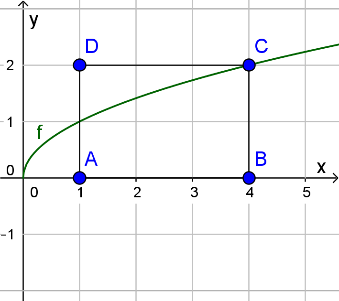
\includegraphics[scale=1.2]{quadratmitwurzel.png}}
		{\begin{tikzpicture}[x=10mm, y=10mm, >=latex, font= \footnotesize, scale=0.9]
				%Raster zeichnen
				\draw [color=gray!50]  [step=10mm] (-1.3,-1.3) grid (5.3,3.3);
				% Achsen zeichnen
				\draw[->,thick] (-1.3,0) -- (5.8,0) node[right, below] {\normalsize $x$};
				\draw[->,thick] (0,-1.3) -- (0,3.8) node[above, left] {\normalsize $y$};
				% Achsen beschriften
				\foreach \x in {-1,1,2,...,5} \draw (\x,-.1) -- (\x,.1) node[below=4pt] {$\x$};
				\foreach \y in {-1,1,2,3} \draw (-.1,\y) -- (.1,\y) node[left=4pt] {$\y$};
				% Besserer Ursprung
				\draw[color=black] (0pt,-7pt) node[right] {$0$};
				%Funktionen zeichnen:
				\clip(-1.3,-1.3) rectangle (5.3,3.3); %Bildbereich
				%Beschriftung
				%\node[myred]  at (3.1,-2.3) {$f$};
		\end{tikzpicture}}
	\end{minipage}
	\begin{parts}
		\setcounter{partno}{2}
		\part Wie berechnest du die Ableitung und die Stammfunktion von f?
		\bl\[F(x)=\frac{2}{3}\*x^\frac{3}{2}+c \qquad f'(x)=\frac{1}{2}\*x^\frac{-1}{2}=\frac{1}{2\*\sqrt{x}}\]\el
		\part Wir wissen von einem Graphen, dass er die $x-$Achse in $x=5$ berührt. Was können wir über die Ableitung und den Graphen aussagen?
		\bl $f'(5)=0$, da die $x-$Achse eine horizontale Tangente ist. Weiter ist $5$ auch eine Nullstelle des Graphen.
		\part Was ist ein Wendepunkt und wie sind sie algebraisch charakterisiert?\\
		Ein Punkt bei den die Krümmung von rechts nach links oder umgekehrt wechselt. Gleichzeitig hat der Graph dort die höchste oder kleinste Steigung\el
	\end{parts}
\end{aufgabe}

%

\bereich{Stochastik}
\titel{Bedingte Wahrscheinlichkeit}
\begin{aufgabe}
	Der Test einer gewissen Krankheit hat eine $98\%$-ige Korrektheit. Das heisst, wenn sich jemand ansteckt wird die Ansteckung in $98\%$ korrekt nachgewiesen.
	\begin{parts}
		\part Benutze das Beispiel oben, um die bedingte Wahrscheinlichkeit zu erklären. Zeige, wo die Wahrscheinlichkeit von $98\%$ im Baum zum Tragen kommt.
		\bl Es ist die Wahrscheinlichkeit, dass ein Event passiert, wenn wir bereits die Kenntnis des vorangegangenen Events haben\el
		\part Wir wissen dass $5\%$ der Bevölkerung an dieser Krankheit leiden und ebenfalls $5\%$ der gesunden Personen ein fälschlicherweise positiven Test erhalten haben. Zeichne diese Informationen zusätzlich oben im Baum ein.
		\bl 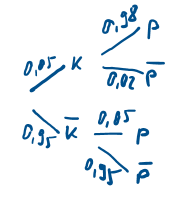
\includegraphics[scale=1]{krankheitsbaum.png}\\
		K heisst krank, p heisst positiver Test \el
		\part Benutze den Baum nun, um die Wahrscheinlichkeit, dass sich einer mit positivem Test infiziert, zu berechnen.
		\bl \[P(K\mid p)=\frac{P(K\cup p)}{P(p)}=\frac{0.05\*0.98}{0.05\*0.98+0.95\*0.05}=0.51\] \el
		\part Betrachte nun einen Würfel und wird diesen $20-$mal. Was ist die Wahrscheinlichkeit, dass wir exakt $7-$mal eine $5$ werfen?
		\bl \[{20\choose 7}\*\left(\frac{1}{6}\right)^7\*\left(\frac{5}{6}\right)^{13}\] \el
		\part Was ist die Wahrscheinlichkeit, dass wir mindestens einmal eine $5$ werfen?
		\bl\[1-{20\choose 0}\*\left(\frac{1}{6}\right)^0\*\left(\frac{5}{6}\right)^{20}\] \el
		\part Was ist die Wahrscheinlichkeit, dass du den Schweizer Lotterie Jackpot knackst, wenn aus $45$ Zahlen genau $6$ richtige aussuchen musst?
		\bl \[\frac{6\*5\*4\*3\*2}{45\*44\*43\*42\*41\*40}\] \el
	\end{parts}
\end{aufgabe}


%----------------------------------------------------------


\bereich{Vektor}
\titel{Koordinatengleichung von Ebenen}
\begin{aufgabe}
	\begin{parts}
		\part Im Allgemeinen: Welche speziellen Eigenschaften besitzen ein gerader Kreiszylinder?
		\bl Ein Kreiszylinder, dessen Mittelpunkte des Bodens bzw. Deckels exakt übereinander liegen. \el
		\part Von einem Zylinder ist das Zentrum ${M(0\mid1\mid1)}$ des Grundflächenkreises, der Punkt\\ ${H(2\mid3\mid0)}$ auf dem Kreis um $M$ liegend und der Punkt ${P(3\mid4\mid2)}$ auf dem \flqq Deckelkreis\frqq\: bekannt. Reichen diese Punkte, um zu überprüfen, ob dies einen geraden Kreiszylinder beschreibt?
		\bl Nein, es reicht nicht. Die Kreise könnten auch verschoben sein. \el
		\part Einer der Kreise des Zylinders liegt auf der Ebene $E:x+y+4z-5=0$. Welcher?
		\bl Füge $H/M$ oder $P$ in $E$ ein und überprüfe. $\Rightarrow M\in E$ \el
		\part Was ist die Gleichung der Ebene, die den anderen Kreis enthält?
		\bl \[x+y+4z+d=0 \Rightarrow P\in E \Rightarrow d=-15\] \el
		\part Wie gross ist das Volumen des Zylinders?
		\bl \begin{align*}
			r&=\abs{\Vec{0}{1}{1}-\Vec{2}{3}{0}}=\sqrt{4+4+1}=3\\
			h&=d(P,E)=\frac{\abs{3+4+8-5}}{\sqrt{9+16+4}}=\frac{10}{\sqrt{29}}\Rightarrow V=1/3\*3^2\*\pi\*\frac{10}{\sqrt{29}}
		\end{align*} \el
		\part Die Ebene $E$ ist in einer Bestimmten Weise gegeben? Welche? Erkläre die Eigenschaften beider Formen und wie du sie bestimmen kannst.
		\bl Koordinatengleichung: Normalvektor und Punkt\\ Parametergleichung: Stützpunkt und zwei nicht kollineare Richtungsvektoren \el
	\end{parts}
\end{aufgabe}

%

\bereich{Differential}
\titel{Kurvendiskussion}
\begin{aufgabe}
	Die Funktion $f(x)=x\*(x+2)\*(x-1)=x^3+x^2-2x$ ist gegeben.\\
	\begin{minipage}{0.6\linewidth}
		\begin{parts}
			\part Skizziere den Graphen der Funktion mit sowenig Aufwand wie möglich. Begründe deine Vorgehensweise.
			\part Füge zusätzlich den Graphen der ersten Ableitung von $f$ ins Koordinatensystem ein.
			\part Erkläre, was ein Wendepunkt ist. Wie können diese Punkte gefunden werden? Warum sind diese Punkte interessant?
			\bl Geometrisch: Krümmungsänderung, steilste Stelle mit pos. or neg. Steigung $\Rightarrow$ Extrema von $f'$\\ Algebraisch: $f'(x)=0 \text{ und } f''(x)\neq0$ \el
		\end{parts}
	\end{minipage}
	\hfill
	\begin{minipage}{0.375\linewidth}
		\ifthenelse{\boolean{printanswers}}
		{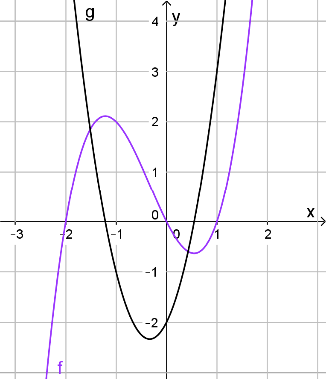
\includegraphics[scale=1.2]{skizzekurvendiskussion.png}}
		{\begin{tikzpicture}[x=10mm, y=10mm, >=latex, font= \footnotesize, scale=0.9]
				%Raster zeichnen
				\draw [color=gray!50]  [step=10mm] (-3.3,-3.3) grid (3.3,5.3);
				% Achsen zeichnen
				\draw[->,thick] (-3.3,0) -- (3.8,0) node[right, below] {\normalsize $x$};
				\draw[->,thick] (0,-3.3) -- (0,5.8) node[above, left] {\normalsize $y$};
				% Achsen beschriften
				\foreach \x in {-3,-2,-1,1,2,3} \draw (\x,-.1) -- (\x,.1) node[below=4pt] {$\x$};
				\foreach \y in {-3,-2,-1,1,2,...,5} \draw (-.1,\y) -- (.1,\y) node[left=4pt] {$\y$};
				% Besserer Ursprung
				\draw[color=black] (0pt,-7pt) node[right] {$0$};
				%Funktionen zeichnen:
				\clip(-3.3,-3.3) rectangle (3.3,5.3); %Bildbereich
				%Beschriftung
				%\node[myred]  at (3.1,-2.3) {$f$};
		\end{tikzpicture}}
	\end{minipage}
	\begin{parts}
		\setcounter{partno}{3}
		\part $g$ sei eine horizontale Linie durch den Wendepunkt. Bestimme die Funktionsgleichung von $g$.
		\bl\begin{minipage}{0.575\linewidth}
			\begin{align*}
				f(x)=x^3+x^2-2x &\Rightarrow f'(x)=3x^2+2x-1\\ f''(x)=6x+2=0 &\Rightarrow x_P=-\frac{1}{3}\\ f(x_P)=\frac{-1}{27}+\frac{1}{9}+\frac{2}{3}&=\frac{20}{27}\Rightarrow g(x)=\frac{20}{27}
			\end{align*}
		\end{minipage}
		\hfill
		\begin{minipage}{0.4\linewidth}
			\begin{tikzpicture}[x=10mm, y=10mm, >=latex, font= \footnotesize, scale=0.8]
				%Raster zeichnen
				\draw [color=gray!50]  [step=10mm] (-3.3,-1.3) grid (3.3,3.3);
				% Achsen zeichnen
				\draw[->,thick] (-3.3,0) -- (3.8,0) node[right, below] {\normalsize $x$};
				\draw[->,thick] (0,-1.3) -- (0,3.8) node[above, left] {\normalsize $y$};
				% Achsen beschriften
				\foreach \x in {-3,-2,-1,1,2,3} \draw (\x,-.1) -- (\x,.1) node[below=4pt] {$\x$};
				\foreach \y in {-1,1,2,...,3} \draw (-.1,\y) -- (.1,\y) node[left=4pt] {$\y$};
				% Besserer Ursprung
				\draw[color=black] (0pt,-7pt) node[right] {$0$};
				%Funktionen zeichnen:
				\clip(-3.3,-1.3) rectangle (3.3,3.3); %Bildbereich
				\draw[plotblue,thick,domain=-3:3,samples=200] plot (\x, {\x*(\x+2)*(\x-1)});
				\draw[myred,thick,domain=-3:3,samples=200] plot (\x, {20/27});
				\draw[fill=charcoal] (-1/3,20/27) circle (1.5pt);
				%Beschriftung
				\node[charcoal]  at (-0.5,0.4) {$P$};
			\end{tikzpicture}
		\end{minipage}\el
		\part Der Graph von $f$ wird nun um zwei Einheiten nach oben geschoben. Wie lautet die neue Funktionsgleichung?
		\bl\[f(x)=x^3+x^2-2x+2\]\el
		\part Wie beeinflusst diese Verschiebung die erste Ableitung von $f$?
		\bl Ableitung verändert sich nicht, da die Gestalt und damit die Steigung nicht verändert wurde.
		\part Wie gross ist die eingeschlossene Fläche zwischen der $x-$Achse und dem Graphen von $f$?
		\[\int_{-2}^{0}f(x)\d{x}+\abs{\int_{0}^{1}f(x)\d{x}}=\left.\frac{1}{4}x^4+\frac{1}{3}x^3-x^2\right\vert_{-2}^0+...\]\el
	\end{parts}
\end{aufgabe}


%----------------------------------------------------------


\bereich{Integral}
\titel{Rotationsvolumen}
\begin{aufgabe}
	\begin{parts}
		\part Ohne irgendwelche Bedingungen skizziere den Graph der Stammfunktion dieser Parabel.
		\ifthenelse{\boolean{printanswers}}
		{\begin{tikzpicture}[x=10mm, y=10mm, >=latex, font= \footnotesize, scale=0.9]
				%Raster zeichnen
				\draw [color=gray!50]  [step=10mm] (-3.3,-3.3) grid (3.3,5.3);
				% Achsen zeichnen
				\draw[->,thick] (-3.3,0) -- (3.8,0) node[right, below] {\normalsize $x$};
				\draw[->,thick] (0,-3.3) -- (0,5.8) node[above, left] {\normalsize $y$};
				% Achsen beschriften
				\foreach \x in {-3,-2,-1,1,2,3} \draw (\x,-.1) -- (\x,.1) node[below=4pt] {$\x$};
				\foreach \y in {-3,-2,-1,1,2,...,5} \draw (-.1,\y) -- (.1,\y) node[left=4pt] {$\y$};
				% Besserer Ursprung
				\draw[color=black] (0pt,-7pt) node[right] {$0$};
				%Funktionen zeichnen:
				\clip(-3.3,-3.3) rectangle (3.3,5.3); %Bildbereich
				\draw[myred,thick,domain=-3:3,samples=200] plot (\x, {1/3*(\x)^3-\x});
				\draw[plotblue,thick,domain=-3:3,samples=200] plot (\x, {(\x)^2-1});
				\draw[plotblue,thick,domain=-3.3:3.3,samples=200] plot (\x, {\x+1});
				%Beschriftung
				\node[myred]  at (3.1,4.8) {$F$};
		\end{tikzpicture}}
		{\begin{tikzpicture}[x=10mm, y=10mm, >=latex, font= \footnotesize, scale=0.9]
				%Raster zeichnen
				\draw [color=gray!50]  [step=10mm] (-3.3,-3.3) grid (3.3,5.3);
				% Achsen zeichnen
				\draw[->,thick] (-3.3,0) -- (3.8,0) node[right, below] {\normalsize $x$};
				\draw[->,thick] (0,-3.3) -- (0,5.8) node[above, left] {\normalsize $y$};
				% Achsen beschriften
				\foreach \x in {-3,-2,-1,1,2,3} \draw (\x,-.1) -- (\x,.1) node[below=4pt] {$\x$};
				\foreach \y in {-3,-2,-1,1,2,...,5} \draw (-.1,\y) -- (.1,\y) node[left=4pt] {$\y$};
				% Besserer Ursprung
				\draw[color=black] (0pt,-7pt) node[right] {$0$};
				%Funktionen zeichnen:
				\clip(-3.3,-3.3) rectangle (3.3,5.3); %Bildbereich
				\draw[plotblue,thick,domain=-3:3,samples=200] plot (\x, {(\x)^2-1});
				\draw[plotblue,thick,domain=-3.3:3.3,samples=200] plot (\x, {\x+1});
				%Beschriftung
				%\node[myred]  at (3.1,-2.3) {$f$};
		\end{tikzpicture}}
		\part Was ist die Fläche, die die beiden Graphen (Parabel und Gerade) einschliessen?
		\bl \begin{align*}
			f(x)=x^2-1 &\Rightarrow F(x)=\frac{1}{3}x^2-x+c \quad g(x)=x+1\\
			\text{Schnittpunkte: } x^2-1=x+1 &\Rightarrow x_{1,2}=\frac{1\pm\sqrt{1+8}}{2}\Rightarrow x_1=2, x_2=-1\\
			\int_{-1}^{2} x+1-(x^2-1)\d{x}&=\left.-\frac{1}{3}x^3+\frac{1}{2}x^2+2x\right\vert_{-1}^2=-\frac{8}{3}+1+4-\left(\frac{1}{3}+\frac{1}{2}+2\right)=4.5
		\end{align*} \el
		\part Die beiden Graphen schneiden sich in zwei verschiedenen Winkeln. Was meinen wir in diesem Fall mit Winkel? Wie würdest du den Winkel beim Punkt $P(2\mid3)$ berechnen?
		\bl Berechne die Steigung der Tangenten an die Parabel im Punkt $P$ danach benutze die Formel... \el
		\part Stell dir vor, die eingeschlossene Fläche der beiden Graphen in ersten Quadranten rotiert um die $x-$Achse. Wie gest du vor, wenn du dieses Rotationsvolumen berechnen möchtest?
	\end{parts}
\end{aufgabe}

%

\bereich{FolgenReihen}
\titel{geometrische Reihe}
\begin{aufgabe}
	\begin{parts}
		\part Gib ein Beispiel einer arithmetischen und einer geometrischen Folge an. Erkläre dabei ihre Eigenschaften.
		\bl AF: Differenz zwischen zwei Gliedern ist konstant\\ GF: Quotient zwischen zwei Gliedern ist konstant \el
		\part Zu welchem Typ von Funktionen sind geometrische resp. arithmetische Folgen verwandt?
		\bl Exponentialfunktionen resp. lineare Funktionen \el
		\part Beschreibe deine Folgen rekursiv und explizit und erkläre die Idee hinter diesen beiden verschiedenen Repräsentationen.
		\bl rekursiv: Beschreibung von einem Element zum nächsten, erstes muss gegeben sein.\\ explizit: Formel wie das $n-$te Glied berechnet wird \el
		\part Wie würdest du die Summe der ersten 20 Glieder am effizientesten bestimmen?
		\bl AF: $\displaystyle s_{20}=\frac{20}{2}(a_1+a_{20})$\\ GF: $\displaystyle s_{20}=a_1\*\frac{1-q^{20}}{1-q}$ \el
		\part Wir kennen die Formel für die unendliche Summe einer geometrischen Folge: $\displaystyle s=a_1\frac{1}{1-q}$. Erkläre in welchen Fällen diese Formel angewendet werden kann.
		\bl Folge muss immer kleiner werden $\Rightarrow \abs{q}<1$ \el
		\part In der Abbildung ist eine Folge von unendlich vielen Halbkreisen mit immer kleiner werdenden Radien abgebildet. Erkläre, wie du die totale markierte Fläche berechnen würdest.
		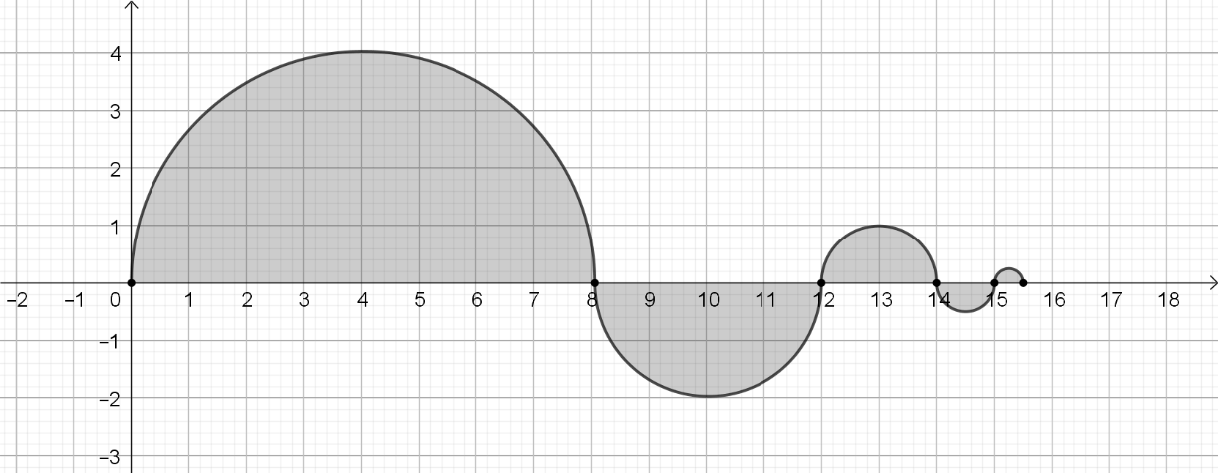
\includegraphics[scale=0.5]{fr-halbkreise.png}
		\bl \begin{align*}
			q_{Radius}&=\frac{1}{2}\\
			q_{Fläche}&=\frac{1}{4}\\
			A_{total}&=a_1\*\frac{1}{1-q_{Fläche}}=\frac{4^2\pi}{2}\*\frac{1}{1-\frac{1}{4}}=...
		\end{align*} \el
	\end{parts}
\end{aufgabe}


%----------------------------------------------------------


\bereich{Integral}
\titel{Stammfunktion}
\begin{aufgabe}
	\begin{minipage}{0.575\linewidth}
		Der Graph recht zeigt die Funktion $f(x)=x\*\sin{x}$.
		\begin{parts}
			\part Erkläre den Ausdruck geometrisch \[\int_{0}^{4}f(x)\d{x}\]
			\bl Die Fläche zwischen Kurve und $x-$Achse. \el
			\part Berechne die Nullstellen der Funktion $f$. Ist das obige Integral positiv oder negativ? Begründe.
			\bl \begin{align*} x\*\sin{x}&=0\\ \Rightarrow x=0\sor\sin{x}&=0 \Rightarrow x=k\*\pi\forall k\in\Z\end{align*}
			Erster Hügel oberhalb heisst positiv danach kleines Stück unterhalb heisst negativ. Insgesamt also nahe bei Null aber vermutlich noch knapp positiv. \el
		\end{parts}
	\end{minipage}
	\hfill
	\begin{minipage}{0.4\linewidth}
		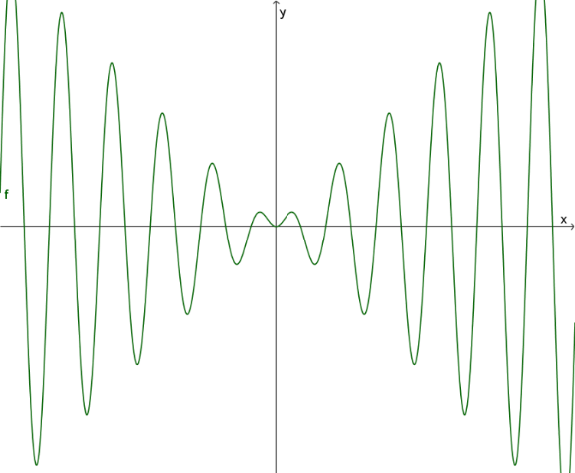
\includegraphics[scale=0.95]{int-oszillierendefunktion.png}
	\end{minipage}
	\begin{parts}
		\part Beweise, dass $F(x)=\sin{x}-x\*\cos{x}$ eine Stammfunktion von $f$ ist.
		\bl \[F'(x)=\cos{x}-(x\*-\sin{x}+1\*\cos{x})=\cos{x}-\cos{x}+x\*\sin{x}=x\*\sin{x}\] \el
		\part Der Graph der Funktion $f(x)=x\*\sin{x}$ ist achsensymmetrisch zur $y-$Achse. Welche Symmetrie würdest du für den Graphen von $g(x)=x\*\cos{x}$ erwarten? Begründe.
		\bl Punktsymmetrisch - da $x$ punktsymmetrisch ist und $\cos{x}$ achsensymmetrisch haben wir verschiedene Vorzeichen rechts und links von der $y-$Achse \el
	\end{parts}
\end{aufgabe}

%

\bereich{FolgenReihen}
\titel{Geometrische Folge}
\begin{aufgabe}
	Es sind drei verschiedene Folgen gegeben: \begin{itemcols}[3]
		\item $4,-6,-16,-26,\ldots$
		\item $4,-1,\frac{1}{4},\frac{-1}{16},\ldots$
		\item $1,2,4,7,11,16,\ldots$
	\end{itemcols}
	\begin{parts}
		\part Finde für jede dieser Folgen eine allgemeine Beschreibung.
		\bl \begin{itemcols}[3]
			\item[ ] $a_n=4-(n-1)\*10$
			\item[ ] $a_1=4,\:a_{n+1}=a_n-10$
			\item[ ] $a_n=4\*\left(\frac{-1}{4}\right)^{n-1}$
			\item[ ] $a_1=4,\: a_{n+1}=a_n\*\frac{-1}{4}$
			\item[ ] $a_1=1,\: a_{n+1}=a_n+n$
		\end{itemcols}\vspace{0.1cm}\el
		\part Welche der obigen Beschreibungen sind rekursiv und welche sind explizit? Erkläre die Bedeutung und den Unterschied.
		\bl rekursiv: das nächste Glied wird aus dem Vorangegangenen berechnet. Erstes Glied muss bekannt sein.\\ explizit: Formel nur abhängig von $n$ \el
	\end{parts}
	\begin{minipage}{0.6\linewidth}
		\begin{parts}
			\setcounter{partno}{2}
			\part Eine Wand aus Backsteinen wird wie auf dem Bild rechts gebaut. Erkläre, wie unser Wissen über Folgen uns hilft die Frage, wie viele Backsteine für eine Wand mit $100$ Zeilen gebraucht werden, zu beantworten.
			\bl \[s=1+2+3+...+100=\frac{100}{2}(1+100)=5050\] \el
		\end{parts}
	\end{minipage}
	\hfill
	\begin{minipage}{0.375\linewidth}
		\centering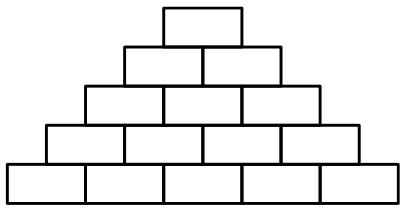
\includegraphics[scale=1]{fr-backsteinmauer.png}
	\end{minipage}
	\begin{parts}
		\setcounter{partno}{3}
		\part Wir nehmen an einen Apfel in einer offenen Schale verliert täglich $2\%$ seiner Masse. Anfangs wog der Apfel $200$g. Benutze eine Folge und eine Funktion, die diesen Zerfallsprozess beschreiben.
		\bl \[a_n=200\*0.98^{n-1} \qquad f(x)=200\*0.98^x\] \el
		\part Skizziere den Graph der Funktion oben in ein Koordinatensystem und kennzeichne die Elemente der Folge.
	\end{parts}
\end{aufgabe}





\bereich{Vektor}
\titel{Geraden}
\begin{aufgabe}
	Gegeben sind zwei Geraden im Raum: \[g:\v{r}=\Vec{-1}{0}{3}+t\*\Vec{0}{1}{1} \qquad h:\v{r}=\Vec{3}{2}{7}+s\*\Vec{6}{-1}{2}\]
	\begin{parts}
		\part Welche Lage können Geraden im Raum zueinander einnehmen?
		\bl identisch, parallel, schneidend und windschief \el
		\part Erkläre, wie du die gegenseitige Lage von $g$ und $h$ findest.
		\bl kollineare Richtungsvektoren? $\Rightarrow$ Nein!\\
		Suche nach gemeinsamen Punkten $\Rightarrow\systeme{-6s=4,t+s=2,t-4s=4}\Rightarrow s=\frac{-2}{3}, t=\frac{8}{3}\Rightarrow S(-1\mid \frac{8}{3}\mid\frac{1}{3})$ \el
		\part Die Gerade $g$ hat eine $0$ im Richtungsvektor. Was können wir daraus über die Position der Gerade aussagen?
		\bl Richtungsvektor zeigt nicht in $x-$Richtung. Das bedeutet, er ist parallel zur $yz-$Ebene. \el
		\part $B(0\mid5\mid0)$ ist ein Punkt der nicht auf der Gerade $g$ liegt. Wir suchen einen Punkt $M$ auf der Gerade $g$, der dem Punkt $B$ am nächsten liegt. Beschreibe deine Vorgehensweise.\\[0.5cm]
		\begin{tikzpicture}[x=10mm, y=10mm, >=latex, font= \footnotesize, scale=1]
			\draw[plotblue,thick] (-3,-3) -- (1,0) node at (-2.75,-2.5) {$g$};
			\draw[fill=charcoal] (0,-2) circle (1.5pt) node[charcoal,below] {$B$};
		\end{tikzpicture}
		\bl 1. $M$ als beliebiger Punkt auf $g$, bestimme den Vektor $\v{BM}$, Skalarprodukt mit Richtungsvektor muss Null sein $\Rightarrow t=\ldots$\\
		2. $M$ ist der Durchstosspunkt, der zur Gerade senkrecht verlaufenden Ebene durch den Punkt $B$. \el
		\part Beschreibe die Ebene die von den beiden Geraden $g$ und $h$ aufgespannt werden. Gib sowohl die Parametergleichung als auch die Koordinatengleichung an.
		\bl Geraden sind schneidend $\Rightarrow$ beide Richtungsvektoren und ein Stützpunkt ergeben\\ Parameterdarstellung $\Rightarrow$ mittels Vektorprodukt dieser beiden Vektoren kann Normalvektor gefunden werden. \el
	\end{parts}
\end{aufgabe}

%

\bereich{Differential}
\titel{Graphen, Spezielle Punkte}
\begin{aufgabe}
	\begin{minipage}{0.6\linewidth}
		\begin{parts}
			\part Der Graph rechts zeigt die Funktionsgraphen der folgenden Funktionen:
			\ifthenelse{\boolean{printanswers}}
			{\begin{itemize}
					\item $\textcolor{forestgreen}{f(x)}=\exp{-x^2}$
					\item $\textcolor{myred}{g(x)}=\frac{1}{2}x^5+3x^3-4x$
					\item $\textcolor{plotblue}{h(x)}=-2(x-1)^2(x+1)$
			\end{itemize}}
			{\begin{itemize}
					\item $f(x)=\exp{-x^2}$
					\item $g(x)=\frac{1}{2}x^5+3x^3-4x$
					\item $h(x)=-2(x-1)^2(x+1)$
			\end{itemize}}
			Ordne die Graphen ihren Funktionsgleichungen zu.
			\part Zwei der Graphen scheinen eine Art Symmetrie aufzuweisen. Wie kann dies aus der Funktionsgleichung abgelesen werden?
			\bl in $f$ wird $x$ quadriert $\Rightarrow$ Vorzeichen spielt keine Rolle\\
			in $g$ sind alle Exponenten ungerade $\Rightarrow$ punktsymmetrisch \el
		\end{parts}
	\end{minipage}
	\hfill
	\begin{minipage}{0.375\linewidth}
		\begin{tikzpicture}[x=10mm, y=10mm, >=latex, font= \footnotesize, scale=0.9]
			%Raster zeichnen
			\draw [color=gray!50]  [step=10mm] (-3.3,-3.3) grid (3.3,3.3);
			% Achsen zeichnen
			\draw[->,thick] (-3.3,0) -- (3.8,0) node[right, below] {\normalsize $x$};
			\draw[->,thick] (0,-3.3) -- (0,3.8) node[above, left] {\normalsize $y$};
			% Achsen beschriften
			\foreach \x in {-3,-2,-1,1,2,...,3} \draw (\x,-.1) -- (\x,.1) node[below=4pt] {$\x$};
			\foreach \y in {-3,-2,-1,1,2,...,3} \draw (-.1,\y) -- (.1,\y) node[left=4pt] {$\y$};
			% Besserer Ursprung
			\draw[color=black] (0pt,-7pt) node[right] {$0$};
			%Funktionen zeichnen:
			\clip(-3.3,-3.3) rectangle (3.3,3.3); %Bildbereich
			\draw[forestgreen,thick,domain=-3:3,samples=200] plot (\x, {exp{-(\x)^2}});
			\draw[myred,thick,domain=-3.3:3.3,samples=200] plot (\x, {1/2*(\x)^5+3*(\x)^3-4*\x});
			\draw[plotblue,thick,domain=-3.3:3.3,samples=200] plot (\x, {-2*(\x-1)^2*(\x+1)});
			%Beschriftung
			%\node[myred]  at (3.1,-2.3) {$f$};
		\end{tikzpicture}
	\end{minipage}
	\begin{parts}
		\setcounter{partno}{2}
		\part Welche speziellen Punkte kannst du im Graphen des \textcolor{plotblue}{blauen} Graphen erkennen?
		\bl Nullstellen, Maximum, Minimum, Wendepunkte \el
		\part Zeige, dass der Ursprung der einzige Wendepunkt der \textcolor{myred}{roten} Funktion ist.
		\bl \begin{align*}
			g'(x)&=\frac{5}{2}x^4+6x^2-4 \qquad g''(x)=10x^3+12x\\
			g''(x)&=0 \Rightarrow x\*(10x^2+12)=0 \Rightarrow\text{Null ist die einzige Lösung!}
		\end{align*}
		\part Da die Nullstellen der \textcolor{myred}{roten} Funktion irrational sind, betrachten wir vereinfacht die Fläche zwischen $x_1=-1$ und $x_2=1$. Berechne sie.
		\begin{align*}
			\int\left(\frac{1}{2}x^2+3x^3-4x\right)\d{x}&=\frac{x^6}{12}+\frac{3x^4}{4}-2x^2\\
			2\*\int_{-1}^{0}\left(\frac{1}{2}x^2+3x^3-4x\right)\d{x}&= 2\*\frac{7}{6} = \frac{7}{3}
		\end{align*}\el
	\end{parts}
\end{aufgabe}


\newpage\ \\
%=========================================================
%-------------------Fragen Hs
%=========================================================
\bereich{Integral}
\titel{Schnittwinkel, Fläche}
\begin{aufgabe}
	Gegeben sind die zwei Funktionsgraphen:\\
	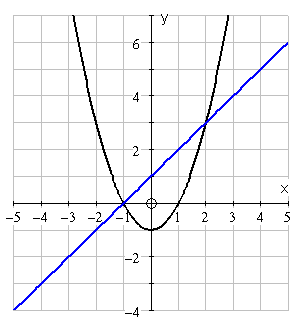
\includegraphics[width=0.4\textwidth]{graph1.png}
	\begin{parts}
		\part Wie lauten die Funktionsgleichungen der abgebildeten Graphen?
		\part Wie bestimmt man die Schnittpunkte?
		\part Was versteht man unter dem Schnittwinkel der Graphen im Schnittpunkt $(2/3)$ und wie müsste man diesen berechnen?
		\part Wie berechnet man die Fläche zwischen den beiden Graphen?
		\bl \part VG: Schnittwinkel, zwei Geraden, Ebenen? Skalarprodukt.
		\el
	\end{parts}
\end{aufgabe}



\end{document}